\documentclass[11pt,a4paper]{article}

%page geometry
\usepackage[margin=0.7in]{geometry}

%encoding
%--------------------------------------
\usepackage[utf8]{inputenc} % input encoding
\usepackage[T1]{fontenc} % output encoding
%--------------------------------------

%French-specific commands
%--------------------------------------
\usepackage{babel}
\usepackage[autolanguage]{numprint}
%--------------------------------------

\usepackage{hyperref}

\usepackage{booktabs}

\usepackage{listings}
\usepackage{color}

\usepackage{graphicx}

\usepackage{caption}
\usepackage{subcaption}

\usepackage{float}


\usepackage{amsmath}
\usepackage{amssymb}

\usepackage[parfill, indent]{parskip}

\usepackage[shortlabels]{enumitem}

\newcommand{\cev}[1]{\reflectbox{\ensuremath{\vec{\reflectbox{\ensuremath{#1}}}}}}

\begin{document}

\title{Game Theory for Image Segmentation}
\author{Clément JAMBON \\ \href{mailto:cjambon@student.ethz.ch}{cjambon@student.ethz.ch}}
\maketitle

\begin{figure}[H]
    \centering
    \begin{subfigure}[b]{0.3\textwidth}
        \centering
        \includegraphics[width=\textwidth]{figures/teaser/hike.jpg}
        \caption{ }
    \end{subfigure}
    \hfill
    \begin{subfigure}[b]{0.3\textwidth}
        \centering
        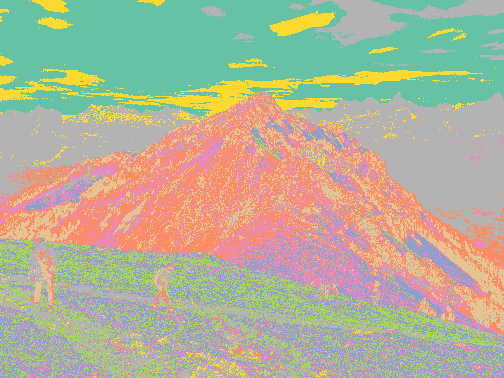
\includegraphics[width=\textwidth]{figures/teaser/hike_seg.png}
        \caption{ }
    \end{subfigure}
    \hfill
    \begin{subfigure}[b]{0.3\textwidth}
        \centering
        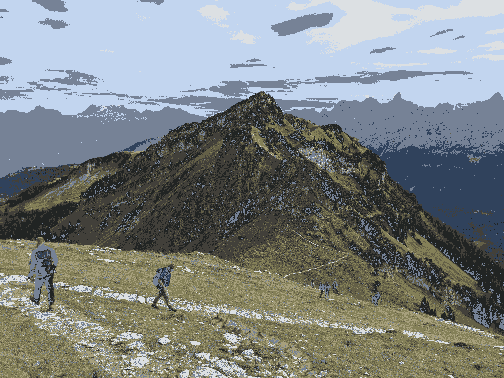
\includegraphics[width=\textwidth]{figures/teaser/hike_avg.png}
        \caption{ }
    \end{subfigure}
       \caption{Segmentation obtained with our implementation of \textit{Pure Infection and immunization dynamics}: (a) is the original image, (b) shows the resulting clusters and (c) the average colors over the segments.}
       \label{fig:teaser}
\end{figure}

\section{Introduction}

Image Segmentation has widely been explored in the Image Processing community. As a consequence, there exists a significant amount of methods including K-Means, graph-based methods\cite{graph-segmentation}, histogram clustering\cite{histogram-clustering} or more recently neural approaches that build on neural networks to extract priors from large amount data\cite{panoptic-segmentation} and allow to cluster pixels beyond color-space similarities.

In this project, motivated by the material of "Controversies in Game Theory"\cite{course-gt}, we choose to focus on another approach that builds on Game Theory and Evolutionary Dynamics. More precisely, inspired by the work of Shen et al.~\cite{game-clustering} and the PhD dissertation of Samuel Rota Bulò\cite{bulo-thesis}, we propose to formulate image segmentation as a clustering game. In order to find the equilibrium of such a game, we lift it to a discrete-time evolutionary dynamics formulation where we make mixed strategies evolve in search for an \textit{Evolutionary Stable Strategy} (ESS). As images are very high-dimensional and lead to slow convergence when using standard algorithms like \textit{Best response dynamics} and \textit{Replicator dynamics}, we follow \cite{game-clustering} and \cite{bulo-thesis}, and use the \textit{Infection and immunization dynamics} with a pure strategy selection function as introduced by Bulò in \cite{inimdyn}. Fig.~\ref{fig:teaser} provides a teaser of our implementation.

We start by reviewing the notion of clustering games with the material from the course\cite{course-gt} in section \ref{sec:cluster-game}. We then introduce discrete-time \textit{Evolutionary dynamics} and the algorithms we use to find such strategies in section \ref{sec:evo-dyn}. This allows us to define Image Segmentation as a clustering game and we present in section \ref{sec:seg-game} our assumptions and experimental setup. Finally, we present our results on RGB similarities in section \ref{sec:results} and propose to extend the method to higher-dimensional features from state-of-the-art deep learning models, namely DINO features\cite{dino} in section \ref{sec:dino}.

Before getting any further, we would like to emphasize that all the results presented in this report were obtained from scratch. Both \cite{bulo-thesis} and \cite{game-clustering} provide a methodology for the described algorithms but we are not aware of any existing implementation. For reproducibility and educational purposes, we make all our code in the form of documented \textit{notebooks} available at \url{https://github.com/clementjambon/evolutionary-segmentation}. 

\section{Clustering game}
\label{sec:cluster-game}

In the following, we introduce the notion of a clustering game and try to stay as close as possible to the notions introduced by Heinrich Nax and Jonny Newton in their lectures from course\cite{course-gt}. In every step, we try to connect the object introduced to the problem of segmentation.

We start by introducing $S=\{1, \ldots, n\}$ a set of \textit{pure strategies} which represent objects to be clustered, in our case image pixels. We connect strategies with a payoff/utility matrix $A$ where $A_{i, j}$ specifies how much one can expect from choosing strategy $i$ against a strategy $j$. In the clustering case, we can interpret this matrix as a similarity matrix that quantifies how close pixel $i$ is similar to $j$. Note that in the following, we will assume only symmetric payoffs (which is consistent to our image-space clustering formulation). 

In practice, we will consider linear combinations $\mathbf{x}$ of these pure strategies as \textit{mixed strategies} that, in order to be consistently comparable, will leave in the $n$-dimensional simplex:
\begin{equation}
    \Delta = \left\{\mathbf{x} = (x_1, \ldots, x_n)\; |\; \sum_{i=1}^n x_i = 1\right\}
\end{equation}
Each mixed strategy comes with a set of non-zero components $\sigma(\mathbf{x})$ which is called its \textit{support}. Intuitively, this will represent a set of pixels belonging to the same cluster. 

With these definitions, we can now see that playing a pure strategy $i$ gives an expected pay-off $\pi(\mathbf{e}_i|\mathbf{x})=\mathbf{e}_i^TA\mathbf{x}$ where $\mathbf{e}_i$ is $i$th vectors of the canonical basis of $\mathbb{R}^n$. More generally, the expected payoff of a mixed strategy $\mathbf{y}$ against another $\mathbf{x}$ is given by $\pi(\mathbf{y}|\mathbf{x})=\mathbf{y}^TA\mathbf{x}$.

As they will be necessary to understand some of the concepts introduced next and in section \ref{sec:evo-dyn}, we also introduce the following notations:
\begin{itemize}
    \item the expected payoff of $\mathbf{x}$ against itself is $\pi(\mathbf{x})=\mathbf{x}^TA\mathbf{x}$
    \item $\pi(\mathbf{y}-\mathbf{x}|\mathbf{x}) = \pi(\mathbf{y}|\mathbf{x}) - \pi(\mathbf{x})$
    \item the \textit{best response} strategies $\beta(\mathbf{x})$ against $\mathbf{x}$ are the strategies that gives the maximum payoff when played against $\mathbf{x}$, namely $\beta(\mathbf{x})=\underset{\mathbf{z}}{\arg\max}\;\pi(\mathbf{y}|\mathbf{x})$. Note that these are not unique!
\end{itemize}

We can now intuitively define the notion of Nash equilibrium with these notations: $\mathbf{x}$ satisfies a \textit{Nash equilibrium} if no other strategies improve its expected payoff against $\mathbf{x}$ than itself or more formally and equivalently (with all the definitions we have):
\begin{equation}
    \forall \mathbf{y}\in\Delta,\quad  \pi(\mathbf{y}|\mathbf{x}) \leq \pi(\mathbf{x}) \iff \forall \mathbf{y}\in\Delta,\quad  \pi(\mathbf{y} - \mathbf{x}|\mathbf{x}) \leq 0 \iff \mathbf{x} \in \beta(\mathbf{x})
\end{equation}

Let's now come back to our clustering game. Intuitively, the goal will be, given a pixel similarity matrix $A$, to find a mixed strategy $\mathbf{x}$ that satisfies a Nash equilibrium and the support of such a strategy will give the pixels classified as part of the same cluster and the remaining pixels will be assigned to another cluster. You may ask now: what if we want to perform clustering with more than 2 clusters? We can simply slice-off the pixels belonging to the first cluster from $S$ and similarity matrix $A$ and find a new Nash equilibrium. In fact, this scheme provides a hint at the strength of clustering game. As emphasized by Bulò in \cite{bulo-thesis}, we need not know the relevant number of cluster in advance, which is a challenging task in Image Segmentation and clustering in general! Instead, we can just run this procedure recursively until $S$ is a singleton or we cannot find a Nash equilibrium (this latter point should not happen with a real symmetric matrix though!). Each of these iterations is called in both \cite{bulo-thesis} and \cite{game-clustering} a \textit{segment}. In practice, as we shall present in section \ref{sec:seg-game}, we define a maximum number of segments in our segmentation case.

\section{Evolutionary dynamics}
\label{sec:evo-dyn}

With the \textit{clustering game} ready, we now need to find how to play the game! More formally, the challenge lies in \textbf{efficiently} finding an equilibrium. To this extent, we follow three approaches from \textit{Evolutionary Dynamics} covered by \cite{bulo-thesis} and \cite{game-clustering}. For conciseness and due to our lack of knowledge on the field, we will only cover the main definitions and give the intuitions behind the corresponding algorithms.

\textit{Evolutionary Dynamics} provides a framework to model the evolution of populations, or in other words mixed strategies, as a function of time. In other words, given an initial mixed strategy $\mathbf{x}^{(0)}$, its evolution  is described as a general differential equation: 
\begin{equation}
    \dot{\mathbf{x}}^{(t)} = g(\mathbf{x}^{(t)}, t)
\end{equation}

In practice, under some assumptions (notably proper renormalization of $\mathbf{x}^{(t)}$), we can discretize this continuous process using discrete time steps $t=1, 2, \ldots$ and express the population $\mathbf{x}^{(t+1)}$ at time $t+1$ as a function of population $\mathbf{x}^{(t)}$ at time $t$.

\subsection*{Best response dynamics}
\textit{Best response dynamics} builds on the intuition that we can inject in the population, at each time step $t$, one individual that would yield the best response w.r.t. the payoff matrix. This gives the following discrete-time dynamics:
\begin{equation}
    \label{eq:best-response}
    \mathbf{x}^{(t+1)} = \frac{ \mathbf{r}^{(t+1)} -  \mathbf{x}^{(t)}}{t + 1} + \mathbf{x}^{(t)} \quad \text{where } \mathbf{r}^{(t+1)}\in\beta(\mathbf{x}^{(t)})
\end{equation}
As the population "grows", the newly added individuals should have less and less of an impact: this is captured by the term $\frac{1}{t}$ in the equation above.

\subsection*{Replicator dynamics}
\textit{Replicator dynamics} are a subset of more general \textit{imitation dynamics}. The key idea is to rescale each entry $i$ of the mixed strategy vector $\mathbf{x}^{(t)}$ at time $t$ depending on how well playing pure strategy $i$ against itself (namely $\mathbf{x}$) performs:
\begin{equation}
    \label{eq:replicator-dynamics}
    x_i^{(t+1)} = x_i^{(t)}\frac{\pi(\mathbf{e}_i|\mathbf{x}^{(t)}) + C}{\pi(\mathbf{x}^{(t)}) + C}
\end{equation}
The constant $C$ is simply introduced to ensure that we do not divide by zero. In our case, as we shall present in section \ref{sec:seg-game}, the similarity matrix has only stricly positive entries and we can just choose $C$ to be zero.

\subsection*{Infection and immunization dynamics}
Unfortunately, \textit{Best response dynamics} and \textit{Replicator dynamics} tend to be particularly slow at approaching an equilibrium (especially when the set of strategies $S$ becomes large which will be a concern to us considering the large number of pixels in an image). See section 3.10 of \cite{bulo-thesis} for a quantitative discussion of this latter point. To address this, Bulò and Bomze introduced in \cite{inimdyn} \textit{Infection and immunization dynamics} (which we further denote as InImDyn for brevity).   

The key takeaway of this more advanced mechanism is, starting from $\mathbf{x}$, to progressively infect the population with another population against which it is not immune. This entails to define the notion of infection and we can naturaly assume that a population $\mathbf{y}$ is \textit{infective} for another population $\mathbf{y}$ if it stricly improves its payoff, namely $\pi(\mathbf{y}|\mathbf{x})>\pi(\mathbf{x})\iff\pi(\mathbf{y}-\mathbf{x}|\mathbf{x})>0$. Following \cite{bulo-thesis}, we denote the corresponding set of infective strategies as $\Upsilon(\mathbf{x})=\{\mathbf{y}\in\Delta\; |\; \pi(\mathbf{y}-\mathbf{x}|\mathbf{x})>0\}$.

However, to actually put into practice such a strategy, two points need to be clarified:
\begin{itemize}
    \item The first is: "which strategy should infect population $\mathbf{x}$?" More formally, we need to define an infective \textit{strategy selection function} $\mathcal{S}(\mathbf{x})$. In \cite{inimdyn}, propose a rather simple idea: find a pure strategy $\mathbf{e}_i$ that maximizes $\pi(\mathbf{e}_i-\mathbf{x}|\mathbf{x})$. Actually, this can be extended further to maximizing $|\pi(\mathbf{e}_i-\mathbf{x}|\mathbf{x})|$ and in the case where this maximum corresponds to a negative value of $\pi(\mathbf{e}_i-\mathbf{x}|\mathbf{x})$ (only allowed when $i$ is in the support of $\mathbf{x}$ to be able to define the \textit{costrategy} thereafter), we can choose what is called the \textit{costrategy} $\bar{\mathbf{e}}_i^\mathbf{x}$ of $\mathbf{e}_i$ w.r.t $\mathbf{x}$ that is obtained by projecting $\mathbf{e}_i$ on the opposite side of the simplex $\Delta$ while passing through $\mathbf{x}$. This can be written analytically as $\bar{\mathbf{e}}_i^\mathbf{x}=-\frac{1}{x_i-1}\mathbf{e}_i+\frac{x_i}{x_i-1}\mathbf{x}$.
    \item The second point is "how much of this selected population $\mathbf{y}=\mathcal{S}(\mathbf{x}^{(t)})$ we should inject within the existing population $\mathbf{x}^{(t)}$ at time $t$. This can be thought of as choosing a nice scalar $\delta_\mathbf{y}(\mathbf{x})$ (similar to $\frac{1}{t+1}$ in eq.~\ref{eq:best-response} describing best response dynamics) such that we can write the discrete update as:
    \begin{equation}
        \label{eq:inimdyn}
        \mathbf{x}^{(t+1)} = \delta_\mathbf{y}(\mathbf{x}) (\mathbf{y} - \mathbf{x}^{(t)}) + \mathbf{x}^{(t)}
    \end{equation}
    By building on the properties of the simplex (we omit the introduction of the notions \textit{score function} and \textit{invasion barriers} to keep the discussion simple) and in the case of our clustering game scenario introduced in section \ref{sec:cluster-game}, one can derive that we can choose (see \cite{bulo-thesis}):
    \begin{equation}
        \delta_\mathbf{y}(\mathbf{x}) = \begin{cases}
            \min\left(\frac{\pi(\mathbf{x}-\mathbf{y}|\mathbf{x})}{\pi(\mathbf{y}-\mathbf{x})}, 1\right) & \text{ if $\pi(\mathbf{y}-\mathbf{x}) < 0$} \\
            1 & \text{ otherwise}
        \end{cases}
    \end{equation}
\end{itemize}

We now mention two results from \cite{bulo-thesis} that hints at the convergence of InImDyn under the pure selection strategy: 
\begin{itemize}
    \item First, Proposition 4 of section 3 of \cite{bulo-thesis} ensures that there exists an infective strategy for a mixed strategy $\textbf{x}$ if and only if the strategy given by the pure strategy selection scheme described above is injective. 
    \item Second, Theorem 2 of section 3 of \cite{bulo-thesis} guarantees that if the set of infective strategies $\Upsilon(\mathbf{x})$ for a population $\mathbf{x}$ is empty, then $\mathbf{x}$ is a fixed point of the InImDyn dynamics and more interestingly a Nash equilibrium.
\end{itemize}

\section{Playing the segmentation game}
\label{sec:seg-game}

With all this nice formalism at our disposal, we now expose how we can use it to practically perform image segmentation. Additionally,we clarify our experimental setup. 

First of all, we need to define the actual payoff matrix $A$. Similar to \cite{bulo-thesis} and \cite{game-clustering}, we choose to compute similarities using a Gaussian Kernel:
\begin{equation}
    A_{i, j}=\exp\left(-\frac{\lVert C(i) - C(j)\rVert^2}{\sigma^2}\right)
\end{equation}
where $C(i)$ corresponds to a 3-dimensional vector representing the value of pixel $i$ in the chosen color space. As suggested in \cite{bulo-thesis}, we convert initial values in \textit{RGB} space to the \textit{Lab} color space using the implementation provided by the OpenCV library\cite{opencv_library}. We choose $\sigma$ to match the dynamic range of standard images, namely $\sigma=250$.

As computations scale quadratically with the side-length of images (because we have $n=H\times W$ pixels), we follow again \cite{bulo-thesis} and subsample pixels at different rates (see next section), run our clustering and then assign out-of-sample pixels using the dominant-set technique from \cite{dominant-set}. In all cases, we initialize the population with $\mathbf{x}^{(0)}$ a constant value (i.e. $\frac{1}{n}$). In other words, all pixels start with an equal probability of belonging to the cluster. We run clustering on at most 8 segments, which yields at most 9 clusters (because we need to account for the potentially non-classified samples at the end of the last segment). For all experiments, we set the maximum number of iterations in a segment to 5000 and stop the dynamics if we a strategy reaches an \textit{$\varepsilon$-neighborhood} of a Nash equilibrium defined in \cite{bulo-thesis} as
\begin{equation}
    \sum_{i=1}^n\left[\min(x_i, \pi(\mathbf{x}-\mathbf{e}_i|\mathbf{x}))\right]^2\leq \varepsilon^2
\end{equation}
and we choose $\varepsilon=10^{-3}$.

Finally, as we try to reproduce the results of \cite{bulo-thesis} and \cite{game-clustering}, we evaluate our algorithms on the BSDS300 dataset\cite{bsds300}.

\section{Results}
\label{sec:results}

All the results provided thereafter can be reproduced by using the notebook provided with this report.

\begin{figure}
    \centering
    \begin{subfigure}[b]{0.3\textwidth}
        \centering
        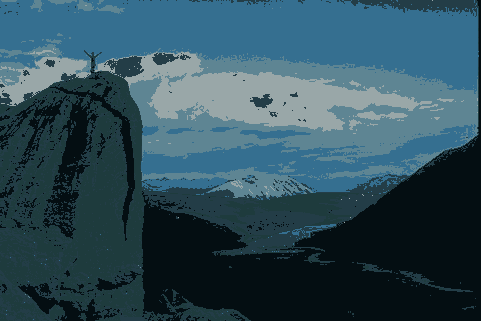
\includegraphics[width=\textwidth]{figures/methods/fp/14037_avg.png}
        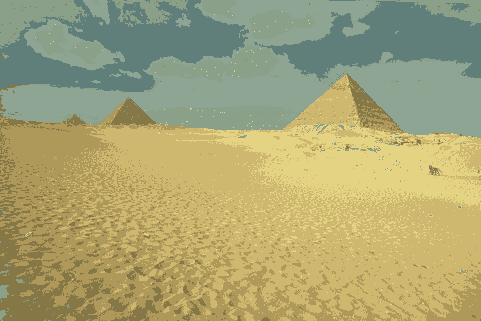
\includegraphics[width=\textwidth]{figures/methods/fp/260058_avg.png}
        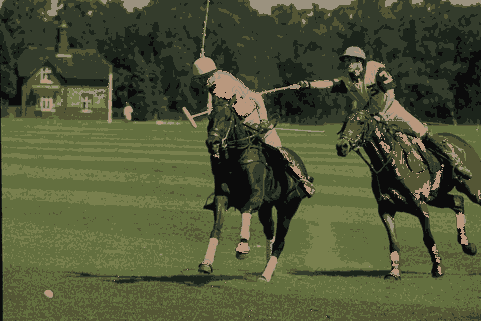
\includegraphics[width=\textwidth]{figures/methods/fp/361010_avg.png}
        \caption{Best Response dynamics}
    \end{subfigure}
    \hfill
    \begin{subfigure}[b]{0.3\textwidth}
        \centering
        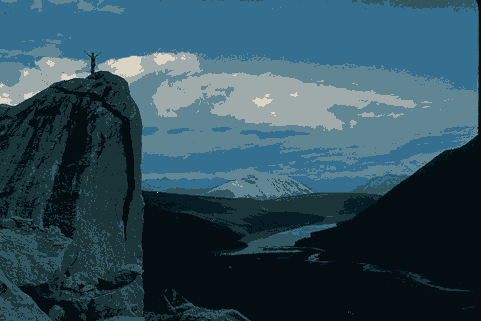
\includegraphics[width=\textwidth]{figures/methods/rd/14037_avg.png}
        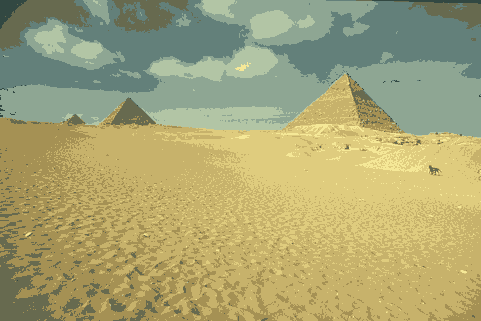
\includegraphics[width=\textwidth]{figures/methods/rd/260058_avg.png}
        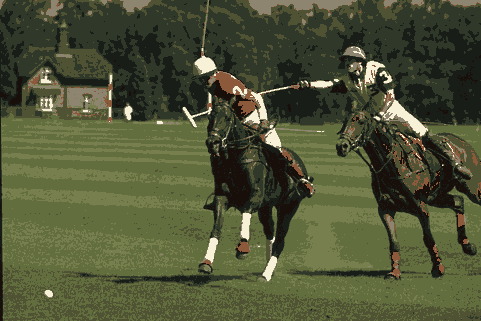
\includegraphics[width=\textwidth]{figures/methods/rd/361010_avg.png}
        \caption{Replicator dynamics}
    \end{subfigure}
    \hfill
    \begin{subfigure}[b]{0.3\textwidth}
        \centering
        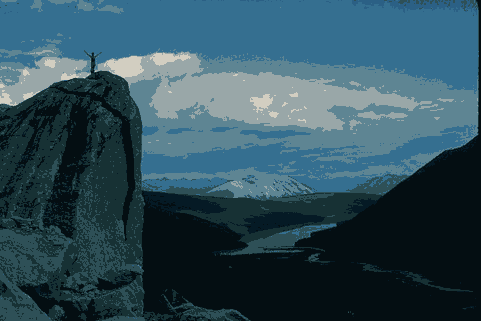
\includegraphics[width=\textwidth]{figures/methods/inimdyn/14037_avg.png}
        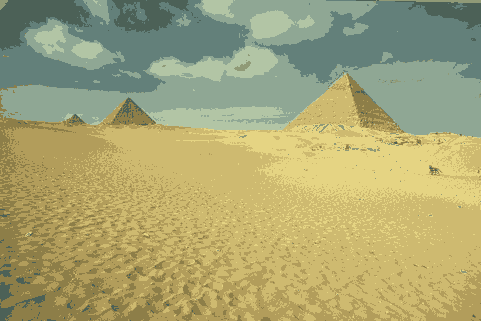
\includegraphics[width=\textwidth]{figures/methods/inimdyn/260058_avg.png}
        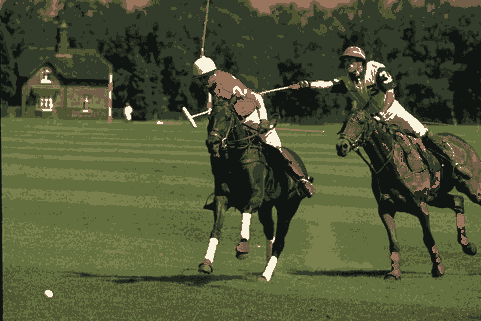
\includegraphics[width=\textwidth]{figures/methods/inimdyn/361010_avg.png}
        \caption{Pure InImDyn}
    \end{subfigure}
       \caption{Segmentations obtained with our implementations of the three dynamics presented in section \ref{sec:evo-dyn} at sampling rate $p=0.01$.}
       \label{fig:results-dynamics}
\end{figure}

In Fig.~\ref{fig:results-dynamics} we compare the three different dynamics on three images from the test set of the BSDS300 dataset. We can clearly see that with a fixed maximum number of iterations, Pure InImDyn clearly outperforms Best Response dynamics. The difference is not so clear for Replicator dynamics. However, as we shall see below, it is significantly more efficiently than the later!

\begin{figure}
    \centering
    \begin{subfigure}[b]{0.24\textwidth}
        \centering
        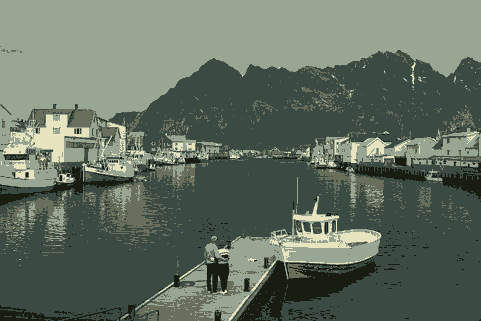
\includegraphics[width=\textwidth]{figures/sampling_rate/0.001/219090_avg.png}
        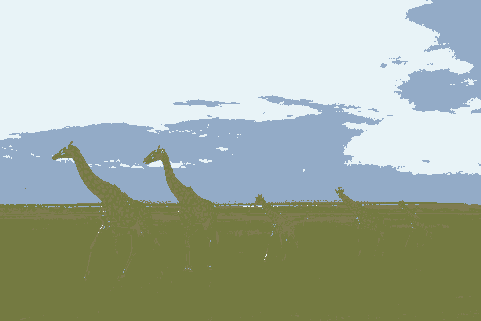
\includegraphics[width=\textwidth]{figures/sampling_rate/0.001/253055_avg.png}
        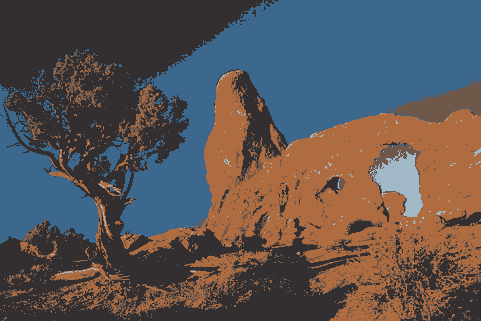
\includegraphics[width=\textwidth]{figures/sampling_rate/0.001/295087_avg.png}
        \caption{$p=0.001$}
    \end{subfigure}
    \hfill
    \begin{subfigure}[b]{0.24\textwidth}
        \centering
        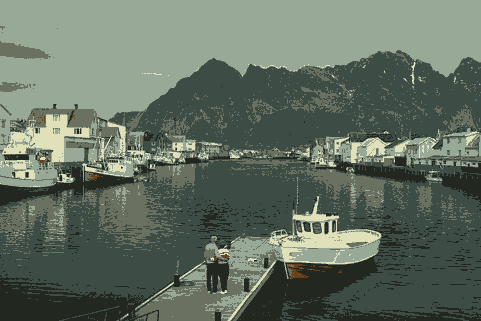
\includegraphics[width=\textwidth]{figures/sampling_rate/0.0025/219090_avg.png}
        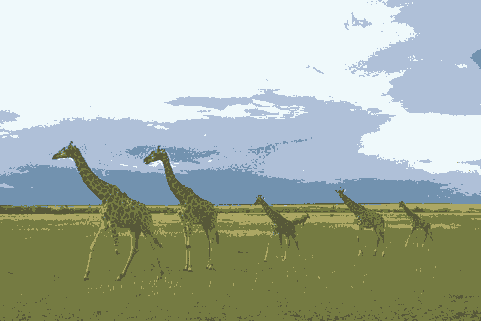
\includegraphics[width=\textwidth]{figures/sampling_rate/0.0025/253055_avg.png}
        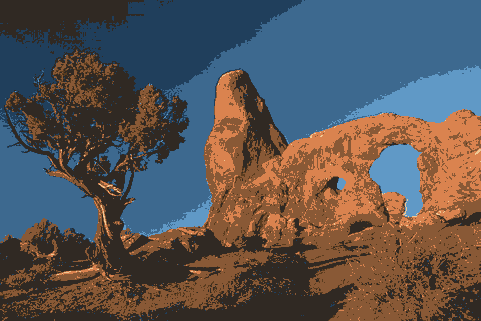
\includegraphics[width=\textwidth]{figures/sampling_rate/0.0025/295087_avg.png}
        \caption{$p=0.0025$}
    \end{subfigure}
    \hfill
    \begin{subfigure}[b]{0.24\textwidth}
        \centering
        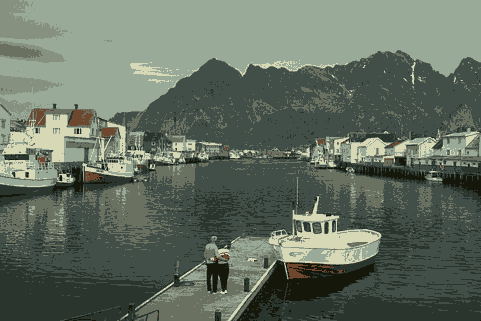
\includegraphics[width=\textwidth]{figures/sampling_rate/0.005/219090_avg.png}
        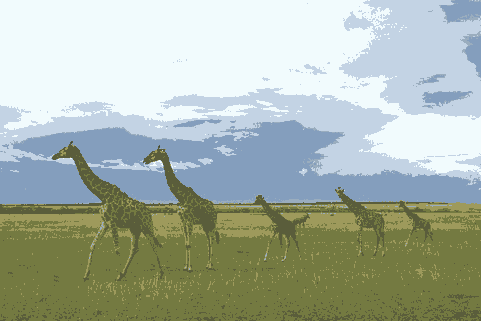
\includegraphics[width=\textwidth]{figures/sampling_rate/0.005/253055_avg.png}
        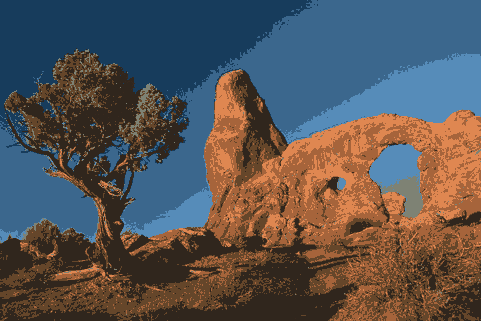
\includegraphics[width=\textwidth]{figures/sampling_rate/0.005/295087_avg.png}
        \caption{$p=0.005$}
    \end{subfigure}
    \begin{subfigure}[b]{0.24\textwidth}
        \centering
        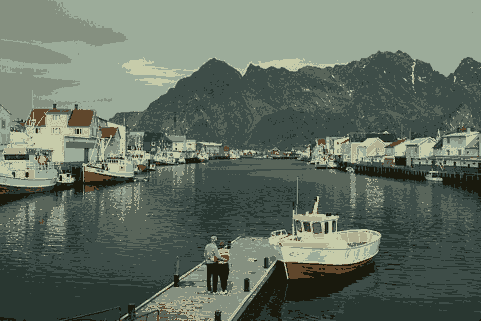
\includegraphics[width=\textwidth]{figures/sampling_rate/0.01/219090_avg.png}
        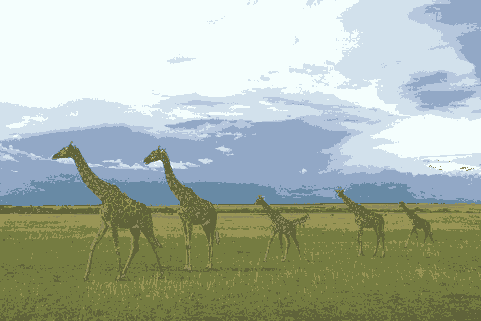
\includegraphics[width=\textwidth]{figures/sampling_rate/0.01/253055_avg.png}
        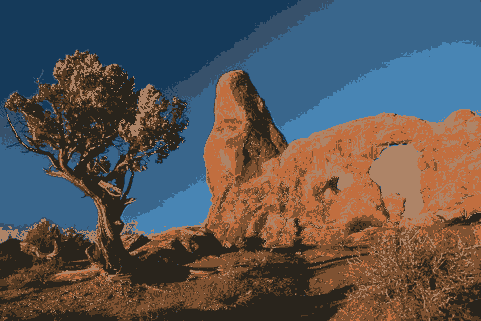
\includegraphics[width=\textwidth]{figures/sampling_rate/0.01/295087_avg.png}
        \caption{$p=0.01$}
    \end{subfigure}
       \caption{Segmentations obtained at different sampling rates.}
       \label{fig:sampling-rate}
\end{figure}

Next, we investigate the impact of the sampling rate $p$. For this, we focus on the InImDyn dynamics. As shown in Fig.~\ref{fig:sampling-rate} and unsurprisingly, higher sampling rates gives perceptually more consistent clusters. However, higher sampling rates require more iterations to converge. This explains the slight decrease in quality between $p=0.005$ and $p=0.01$ in Fig.~\ref{fig:sampling-rate}.

\begin{figure}
    \centering
    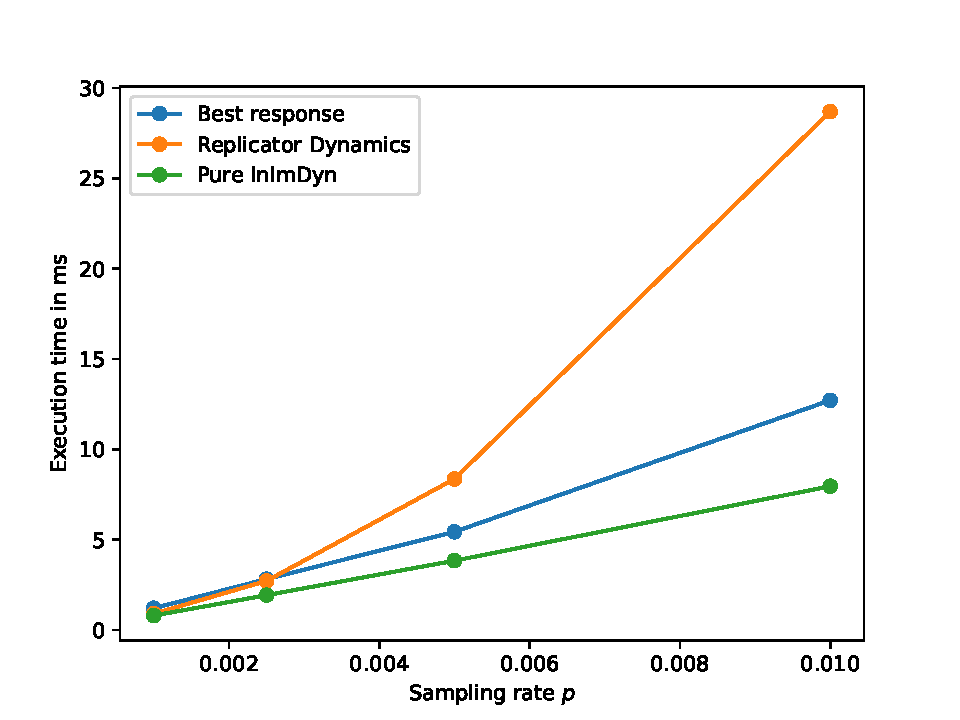
\includegraphics[width=0.7\textwidth]{figures/execution_time.pdf}
    \caption{Average execution time on the test set of the BSDS300 dataset at different sampling rates and across the multiple dynamics}
    \label{fig:execution-time}
\end{figure}

Furthermore, to motivate the advantage of Pure InImDyn over Best Response and Replicator dynamics, we execute our three dynamics on the test set of the BSDS300 dataset and record the execution time. Fig.~\ref{fig:execution-time} shows the significant gain that InImDyn provides us with.

\begin{figure}
    \centering
    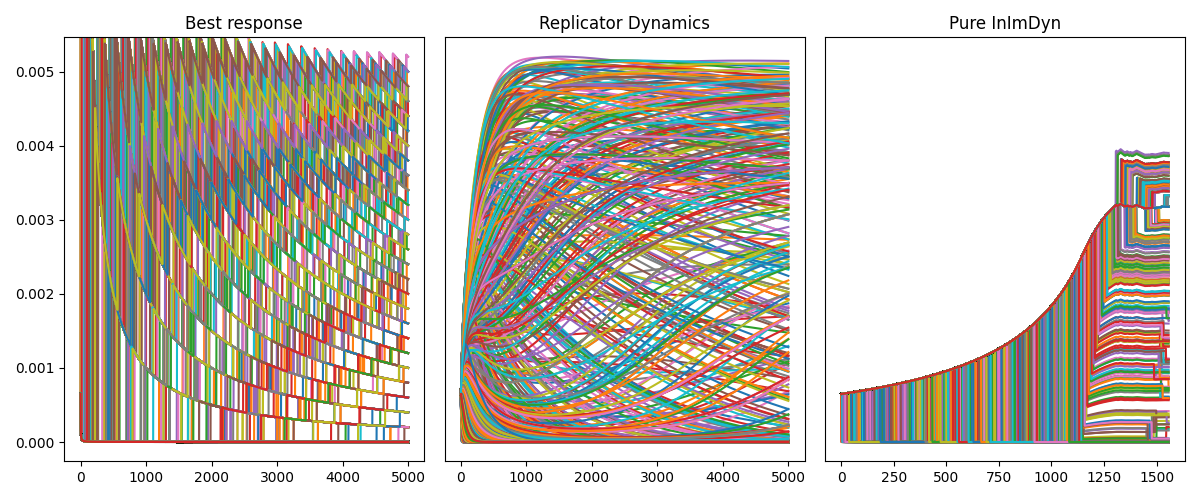
\includegraphics[width=0.8\textwidth]{figures/trajectories/102061.png}
    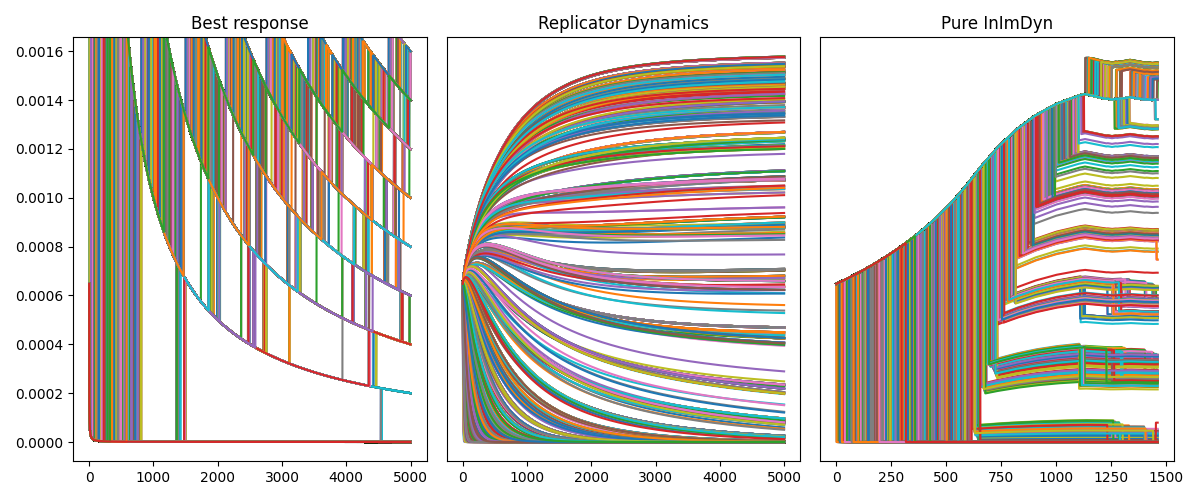
\includegraphics[width=0.8\textwidth]{figures/trajectories/196073.png}
    \caption{Trajectories of the mixed strategy entries on the first segment of two images from the BSDS300 dataset}
    \label{fig:trajectories}
\end{figure}

Finally, we show in Fig.~\ref{fig:trajectories} examples of the distribution of strategies as they evolve following the discrete-time dynamics of each of the investigate approaches. These results are consistent with the one presented in \cite{game-clustering}. We can see in the right column that Pure InImDyn reaches an equilibrium faster than the other dynamics.

\section{Going deeper: \textit{DINO} feature for semantic segmentation}
\label{sec:dino}

\begin{figure}
    \centering
    \begin{subfigure}[b]{0.3\textwidth}
        \centering
        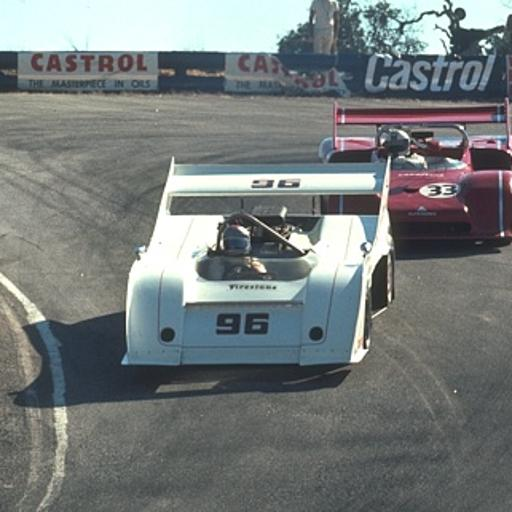
\includegraphics[width=\textwidth]{figures/dino/tile_1/21077.jpg}
        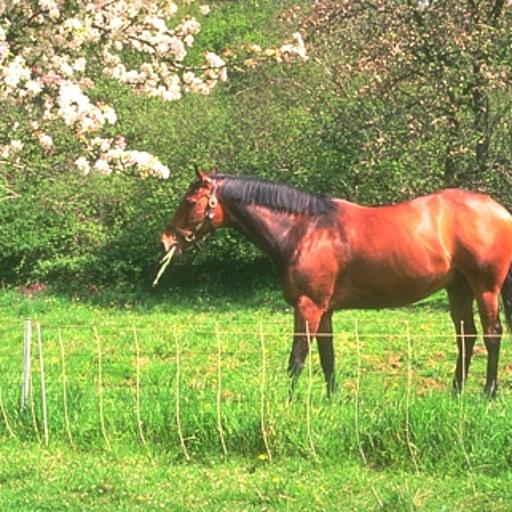
\includegraphics[width=\textwidth]{figures/dino/tile_1/291000.jpg}
        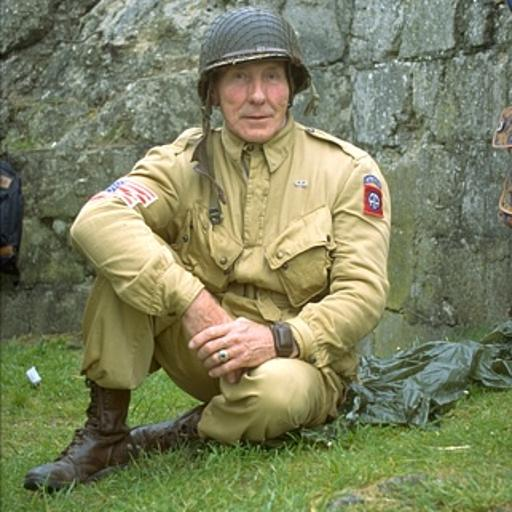
\includegraphics[width=\textwidth]{figures/dino/tile_1/376043.jpg}
        \caption{Original}
    \end{subfigure}
    \hfill
    \begin{subfigure}[b]{0.3\textwidth}
        \centering
        
\includegraphics[width=\textwidth]{figures/dino/tile_1/21077_seg.png}
        
\includegraphics[width=\textwidth]{figures/dino/tile_1/291000_seg.png}
        
\includegraphics[width=\textwidth]{figures/dino/tile_1/376043_seg.png}
        \caption{Clusters}
    \end{subfigure}
    \hfill
    \begin{subfigure}[b]{0.3\textwidth}
        \centering
        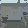
\includegraphics[width=\textwidth]{figures/dino/tile_1/21077_avg.png}
        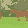
\includegraphics[width=\textwidth]{figures/dino/tile_1/291000_avg.png}
        
\includegraphics[width=\textwidth]{figures/dino/tile_1/376043_avg.png}
        \caption{Average colors}
    \end{subfigure}
       \caption{Segmentations obtained with DINO features on $28\times 28$ feature maps.}
       \label{fig:results-dino}
\end{figure}

\begin{figure}
    \centering
    \begin{subfigure}[b]{0.3\textwidth}
        \centering
        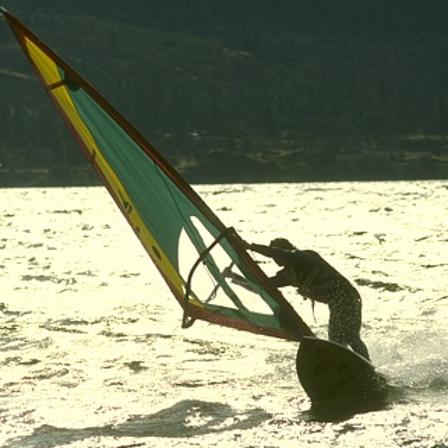
\includegraphics[width=\textwidth]{figures/dino/tile_2/62096.jpg}
        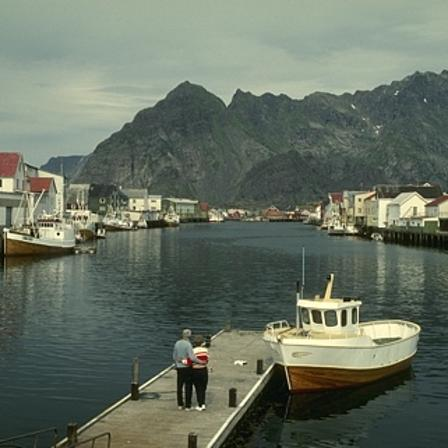
\includegraphics[width=\textwidth]{figures/dino/tile_2/219090.jpg}
        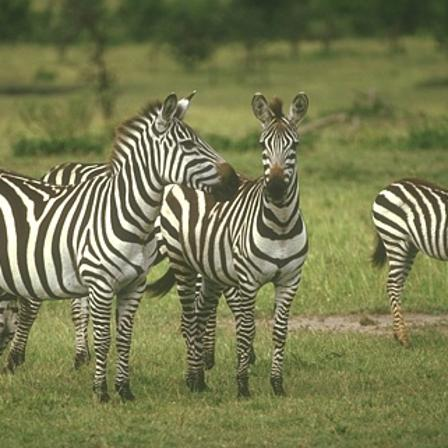
\includegraphics[width=\textwidth]{figures/dino/tile_2/253027.jpg}
        \caption{Original}
    \end{subfigure}
    \hfill
    \begin{subfigure}[b]{0.3\textwidth}
        \centering
        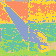
\includegraphics[width=\textwidth]{figures/dino/tile_2/62096_seg.png}
        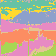
\includegraphics[width=\textwidth]{figures/dino/tile_2/219090_seg.png}
        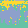
\includegraphics[width=\textwidth]{figures/dino/tile_2/253027_seg.png}
        \caption{Clusters}
    \end{subfigure}
    \hfill
    \begin{subfigure}[b]{0.3\textwidth}
        \centering
        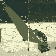
\includegraphics[width=\textwidth]{figures/dino/tile_2/62096_avg.png}
        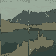
\includegraphics[width=\textwidth]{figures/dino/tile_2/219090_avg.png}
        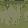
\includegraphics[width=\textwidth]{figures/dino/tile_2/253027_avg.png}
        \caption{Average colors}
    \end{subfigure}
       \caption{Segmentations obtained with DINO features on $4$ tiles of $28\times 28$.}
       \label{fig:results-dino-tile2}
\end{figure}

Motivated by the advent of deep learning and the more interesting task of \textit{semantic segmentation}, we propose an attempt to extend the method to tackle the latter problem using \textit{DINO} features. These high-dimensional features were introduced by Caron et al.~ in \cite{dino}. They result from a self-supervised training procedure with Vision Transformers\cite{transformers}. Most importantly to us, they were shown to embed semantic information. We thus investigate whether we can repurpose our segmentation algorithm from RGB space to this high-dimensional space.

First of all, we extract DINO features using the \href{https://huggingface.co/facebook/dino-vitb8}{facebook/dino-vitb8} model available on \url{https://huggingface.co/}{huggingface}. This model assumes images of size $224\times 224$ and produces features of dimension $768$ by considering patches of 8 pixels. This results in $28\times 28$ images, which is significantly low resolution but still provides us with a coarse semantic segmentation in the end. Additionally, we propose alternative results where we tile the image into 4 blocks of $224\times 224$ thus doubling the size of the result. Yet due to the receptive field of the network, this results in artifacts at the junction of the tiles. As $768$ is a very high dimension, we run a PCA on the features to reduce their dimensionality to 64 only.

In order to run our segmentation algorithm, we modify the similarity matrix to account for the high dimensionality of the DINO features. Instead of a L2 loss, we consider cosine similarities, thus redefining $A$ with $A_{i, j}=\exp\left(-\frac{(1-\text{sim}(\phi_i, \phi_j))}{T}\right)$ where $\text{sim}$ stands for the cosine similarity between the features $\phi_i$ (resp. $\phi_j$) from pixel $i$ (resp. $j$) and $T$ is a temperature parameter. In our experiments, we chose $T=25$.

Fig.~\ref{fig:results-dino} (resp. Fig.~\ref{fig:results-dino-tile2} ) shows the results of segmentation with 1 (resp. 4 tiles).Despite the rather low image size of the DINO feature maps, we can clearly segment semantically the input images. I find it particularly interesting that we managed to adapt a decade-old algorithm to state-of-the-art methods in a conclusive manner.

\section{Conclusion and discussion}

In this project, we investigated a game theoretic approach to Image Segmentation. To do so, we built on the previous works \cite{bulo-thesis} and \cite{game-clustering}, and proposed to study three different evolutionary dynamics: \textit{Best Response dynamics}, \textit{Replicator dynamics} and \textit{Infection and immunization dynamics} with a pure selection strategy. Consistently with their results, we showed that InImDyn provides a good tradeoff between efficiency and quality (in terms of equilibrium).

Our clustering game is very simple and only rely on pairwise similarities between pixels without taking into account spatiality or any form of aggregated payoff. As a consequence, it would be interesting to study higher-order similarities as introduced later in Bulò's PhD dissertation\cite{bulo-thesis}.

\bibliographystyle{plain}
\bibliography{biblio}

\end{document} 
